% JESUS IS LORD

%........................................
\documentclass{article}
\usepackage{graphicx} % Required for inserting images
\usepackage{tabularx}
\usepackage{blindtext}
%\userpackage{parskip}
\usepackage[a4paper, total={7.5in, 10in}]{geometry}
\usepackage{comment}
\usepackage{caption}
\usepackage{subcaption}
\usepackage{amsfonts}
\usepackage{hyperref}  % Add this package in the preamble
\usepackage{geometry}
\usepackage{multirow}
\usepackage{mathtools}
\usepackage{amsmath}
\usepackage{cancel}



\title{Derivations For The Linear Density Wave Model (Victor Afigbo) \\[0.5ex] \large}

\begin{document}
%........................................
\maketitle

%........................................................................
\subsubsection{The Theory of Spiral Density Waves: Linear Density Wave Model}
In this section, we outline the concept of spiral density waves, how it is formed across Saturn's C ring and the mathematical representation of such phenomenon.
Basically, when normal-mode oscillations take place within gaseous planets, like Saturn, they do so in terms of vibrations, and these vibrations in turn give rise to variations in density within the planet, causing disturbances to be generated within the planet, and these disturbances in turn propagate towards the exterior of Saturn. Saturn's gravitational field simply couples these disturbances to the plane of the rings, and these disturbances travel across the stretch of the ring in form of density waves, spiral density and spiral bending waves. Our main focus is on the spiral density waves since their main cause are as a result of normal mode excitation within Saturn.


For a better understanding of this work on the spiral density wave analysis, we need to outline the theory behind the algorithms used in the subsequent sections.
Here, we are utilizing the density wave model to produce anticipated wave profiles \cite{Nicholson1990AnAR}. The specific model we are using is the linear, damped model which was originally derived and elaborately introduced by Shu in 1984 \cite{article}. To provide the essential details for our project, we will give a concise explanation of the model equations as well as the model parameters. This will help us to understand the workings of the model better and enable us to use it more effectively in our project. The linear, damped model is a well-established method that has been utilized in many scientific studies to describe a variety of astronomical phenomena.

Usually, when these waves are propagated across the ring, they are displayed as fluctuations in the density of the ring's surface, which affects its optical properties. This fluctuation has an m-fold symmetry and rotates with respect to the fixed reference frame at a rate of $\Omega_{p}$. The altered surface density distribution, normalized to the background density in areas outside the waves' region, $\sigma_{0}$, is represented by the expression \cite{Nicholson1990AnAR}:

\vspace{2}

\begin{equation}
\Delta \sigma(r,\lambda,t) = 1 + \Re\{-iA_{L}[\pi^{-1/2}-2i\xi H(\xi)]e^{i\phi}\}e^{-(\xi /\xi_{D})^{3}},
\end{equation}
The wave phase, $\phi$, and dimensionless distance from the resonance location, $\xi$, are clearly defined in the equations below, alongside $\xi_{D}$, which denotes the characteristic damping length of the wave. 

\vspace{2}
Simplifying the previous equation using Euler's identify, we have the variant below:
\begin{equation}
\Delta \sigma(r,\lambda,t) = 1 + \Re\{A_{L}e^{i(\phi-\pi/2)}[\pi^{-1/2}+2\xi e^{-i\pi/2}H(\xi)]\}e^{-(\xi/\xi_{D})^{3}}
\end{equation}

\vspace{2}

The function $H(\xi) = \pi^{-1/2}e^{-i\xi^{2}}\int_{-\infty}^{\xi}e^{i\eta^{2}}d\eta$. $H(\xi)$ includes the Standard Fresnel integral. Let $H(\xi) = \pi^{-1/2}e^{-i\xi^{2}}\gamma(\xi)$, so that the Standard Fresnel integral, $\gamma(\xi)$, is excluded from the function, $H(\xi)$. Thus we have the expression below:
\begin{equation}
    \gamma(\xi) = \int_{-\infty}^{\xi}e^{i\eta^{2}}d\eta
\end{equation}


Far into the region of wave propagation, $\xi$ is considered large and positive  \cite{Nicholson1990AnAR} \cite{1984prin.conf..513S}. Also considering the notion that the complex-Gaussian expression is exponentially convergent, we can simply separate the aforesaid integral for easy analysis resulting to the expression,
\begin{equation}
    \gamma(\xi) = \int_{-\infty}^{+ \infty}e^{i\eta^{2}}d\eta - \int_{\xi}^{\infty}e^{i\eta^{2}}d\eta = \gamma_{1} + \gamma_{2}
\end{equation}

\textbf{First Part of Integral:}
Here in this section, we are going to resolve the first part of the expanded integral for $\gamma(\xi)$, using contour integration. Let $\gamma_{1} = \int_{-\infty}^{+ \infty}e^{i\eta^{2}}d\eta$ and $\gamma_{2} = - \int_{\xi}^{\infty}e^{i\eta^{2}}d\eta$.

Considering $\gamma_{1}$, and since it is similar to the real Gaussian function, we devise a technique along the lines of Contour integration to bring it closer to the real Gaussian expression for easy analysis. Let,
\begin{equation}
    \gamma_{1} = \int_{-\infty}^{+ \infty}e^{i\eta^{2}}d\eta = 2\int_{0}^{+ \infty}e^{-(-i\eta^{2})}d\eta.
\end{equation}
Using polar coordinate expression for the arguments of $\gamma_{1}$, we have this as:
\begin{equation}
    \gamma_{1} = 2\int_{0}^{+ \infty}e^{-(e^{-i\pi/2} \eta^{2})}d\eta.
\end{equation}
We go on to factorize the previous equation and this results to, 
\begin{equation}
    \gamma_{1} = 2\int_{0}^{+ \infty}e^{-(e^{-i\pi/4} \eta)^{2}}d\eta.
\end{equation}
By substituting a variable for the exponential argument, we let $\rho = e^{-i\pi/4} \eta$ \cite{video}. Reshuffling the limits of our integral, we have: 
\begin{equation}
    \gamma_{1} = 2 e^{i\pi/4} \lim_{{R \to \infty}} \int_{0}^{Re^{-i\pi/4}} e^{-(\rho)^{2}} \, d\rho
\end{equation}

Let $\gamma_{1}^{'}$ represent the coefficient of 2 and the Euler argument in the main expression for $\gamma_{1}$, we have this as: $\gamma_{1}^{'} = \lim_{{R \to \infty}} \int_{0}^{Re^{-i\pi/4}} e^{-(\rho)^{2}} \, d\rho$, hence $\gamma_{1} = 2 e^{i\pi/4} \gamma_{1}^{'}$.

%............................................
\begin{figure}[h] 
\centering
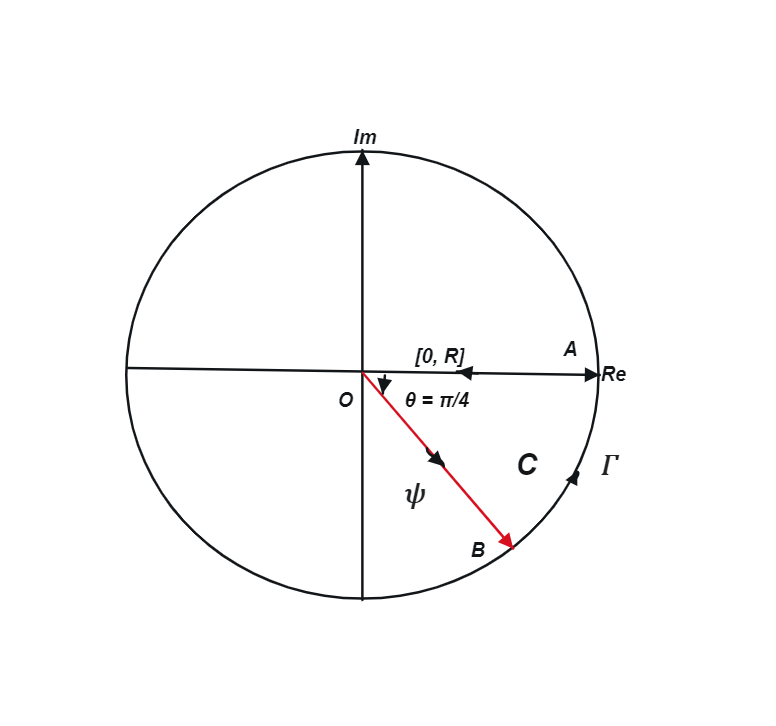
\includegraphics[width=0.8\textwidth]{COUNTOUR_INTEGRATION_DIAGRAM.png}
\caption{ Description of a pizza-shaped contour, consisting of the real (horizontal) and imaginary (vertical) axis.} \label{fig:my_label}
\end{figure}
%............................................

Considering the closed contour, as given in the diagram, for a pizza-shaped type of contour slice at an angle of $\pi/4$ radian (this angle also buttresses the asymptotic nature of $\xi$ \cite{Tiscareno_2007}), we can parametrize the previous expression and go on to evaluate the exact value of the Fresnel integral. This simply allows us to decomposed our contour integration according to the three sections present in our defined contour using complex analysis notations,
\begin{equation}
    \oint_{C} e^{-(z)^{2}} \, dz = \int_{\Psi} e^{-(z)^{2}} \, dz + \int_{\Gamma} e^{-(z)^{2}} \, dz + \int_{R}^{0} e^{-(z)^{2}} \, dz.
\end{equation}


Using Cauchy-Riemann's theorem, $\oint_{C} e^{-(z)^{2}} \, dz = 0$ (on the left hand side of the equation), since it is holomorphic inside and on $C$. Next, we consider the three sections of the given contour.

Given the conditions, $C = \left\{ z = x : 0 \leq x \leq R \right\} \cup \left\{ z : z = Re^{i\theta}, -\frac{\pi}{4} \leq \theta \leq 0 \right\} \cup \left\{ z : z = r,  0 \leq r \leq Re^{-i\frac{\pi}{4}}\right\}$, we can start with the line segment OB, $\Psi$. Here, 
\begin{equation}
    \int_{\Psi} e^{-(z)^{2}} \, dz = \int_{0}^{Re^{-i\frac{\pi}{4}}} e^{-(r)^{2}} \, dr.
\end{equation}
As $R \rightarrow \infty$, the integral along $\Psi$ assumes the format of a typical Gaussian integral, hence $\int_{0}^{\infty} e^{-(r)^{2}}\, dr = \frac{\sqrt{\pi}}{2}$.

Considering the arc BA, corresponding to the section $\Gamma$ of our contour integration,
\begin{equation}
    \int_{\Gamma} e^{-(z)^{2}} \, dz = \int_{-\frac{\pi}{4}}^{0} e^{-(z)^{2}} \, dz, \hspace{3} dz = iRe^{i\theta} d \theta. 
\end{equation}
By substitution we have the form for $\Gamma$ as,
\begin{equation}
    \int_{\Gamma} e^{-(z)^{2}} \, dz = \int_{-\frac{\pi}{4}}^{0} e^{-R^{2}e^{2i\theta}} iRe^{i\theta} d\theta. 
\end{equation}
Considering the absolute value of the given integral along the arc, $\Gamma$, this can be written as:
\begin{equation}
   \left| \int_{\Gamma} \right| \leq \int_{-\frac{\pi}{4}}^{0} \left|e^{-R^{2}e^{2i\theta}} iRe^{i\theta}\right| d\theta = R\int_{-\frac{\pi}{4}}^{0} \left|e^{-R^{2}e^{2i\theta}}\right| d\theta = R\int_{-\frac{\pi}{4}}^{0} \left|e^{-R^{2}[{\cos{(2\theta)} + i\sin{(2\theta)}}]}\right| d\theta.
\end{equation}
Using Euler's indentity, we reduce the expression to its real part only,
\begin{equation}
   \left| \int_{\Gamma} \right| \leq R\int_{-\frac{\pi}{4}}^{0}e^{-R^{2}\cos(2\theta)}d\theta.
\end{equation}
Intuitively, an integral like the one above with such property, vanishes as R becomes large. We are going to validate this claim analytically. A plot of $\cos(2\theta)$ $\forall \theta \in [-\frac{\pi}{4}, 0]$ simply shows that it has its minimum point at $-\frac{\pi}{4}$ and maximum point at $0$. We actually need a function within the same bound that best maximizes the $\cos(2\theta)$ within the exponential argument, to help validate our claim. An optimized function for this operation is $f(\theta) = \frac{4\theta}{\pi}+1$. This implies that, $\cos(2\theta) \geq f(\theta), \forall \theta \in [-\frac{\pi}{4}, 0]$.
Therefore, $e^{-R^{2}\cos(2\theta)} \leq e^{-R^{2}(\frac{4\theta}{\pi}+1)}$. Applying this to the previous case, 
\begin{equation}
   \left| \int_{\Gamma} \right| \leq R\int_{-\frac{\pi}{4}}^{0}e^{-R^{2}(\frac{4\theta}{\pi}+1)}d\theta = \frac{\pi}{4R}(1 - e^{-R^{2}})
\end{equation}
So we establish that, 
\begin{equation}
\lim_{{R \to \infty}} \left| \int_{\Gamma} \right| = \lim_{{R \to \infty}} \frac{\pi}{4R}(1 - e^{-R^{2}}) \leq 0.
\end{equation}

Next, we consider line segment OA, the real part of the contour. Redirecting the integral expression for that section, we have:
\begin{equation}
 \lim_{{R \to \infty}} \int_{R}^{0} e^{-(z)^{2}} \, dz = \lim_{{R \to \infty}} - \int_{0}^{R} e^{-(x)^{2}} \, dx = - \int_{0}^{\infty} e^{-(x)^{2}} \, dx = -\frac{\sqrt{\pi}}{2}.
\end{equation}

Recall, $\oint_{C} e^{-(z)^{2}} \, dz = \int_{\Psi} e^{-(z)^{2}} \, dz + \int_{\Gamma} e^{-(z)^{2}} \, dz + \int_{R}^{0} e^{-(z)^{2}} \, dz.$ Using the answers to each integral, $0 = \frac{\sqrt{\pi}}{2} + 0 - \frac{\sqrt{\pi}}{2}$, which is \textbf{true}. This shows that, $\gamma_{1}^{'} = \frac{\sqrt{\pi}}{2}$ and $\gamma_{1} = \sqrt{\pi}e^{i\pi/4}$.

\vspace{3}

\textbf{Second Part of Integral:}
For the case of $\gamma_{1}$, we could decompose it into a standard Fresnel integral and an integral that behaves like a Fresnel function as its argument approaches infinity. Here,
\begin{equation}
\gamma_{2} = - \int_{\xi}^{\infty}e^{i\eta^{2}}d\eta = -\int_{0}^{\infty}e^{i\eta^{2}}d\eta + \int_{0}^{\xi}e^{i\eta^{2}}d\eta = -\frac{\sqrt{\pi}}{2}e^{i\frac{\pi}{4}} + \int_{0}^{\xi}e^{i\eta^{2}}d\eta.
\end{equation}
Using the de Moivre's theorem, $\int_{0}^{\xi}e^{i\eta^{2}}d\eta = \int_{0}^{\xi}[cos(\eta^{2}) + isin(\eta^{2})]d\eta$. Let $C(\xi) = \int_{0}^{\xi}\cos(\eta^{2})d\eta$ and $S(\xi) =  \int_{0}^{\xi}\sin(\eta^{2})d\eta$ assume the real and imaginary parts of the asymptotic Fresnel expressions, respectively, so that $\int_{0}^{\xi}e^{i\eta^{2}}d\eta = C(\xi) + iS(\xi)$.

\vspace{5}

We can express the asymptotic behaviour of the aforesaid Fresnel integrals using the given forms as \cite{abramowitz1968handbook}\cite{enwiki:1181389148}\cite{wolfram-alpha-notebook}: 
\begin{equation}
C(\xi) = \sqrt{\frac{\pi}{8}}\,\text{sgn}(\xi) + \left[1 + O\left(\xi^{-4}\right)\right]\left(\sin(\xi^2)\left(\frac{1}{2\xi}\right) + \cos(\xi^2)\left(-\frac{1}{4}\,O\left(\xi^{-3}\right)\right)\right)
\end{equation}
and
\begin{equation}
S(\xi) = \sqrt{\frac{\pi}{8}}\,\text{sgn}(\xi) - \left[1 + O\left(\xi^{-4}\right)\right]\left(\cos(\xi^2)\left(\frac{1}{2\xi}\right) + \sin(\xi^2)\left(\frac{1}{4}\,O\left(\xi^{-3}\right)\right)\right).
\end{equation}


In the case of our model, we assume a moderate propagation of the density waves, which implies that as $\xi \rightarrow \infty$, $\mathcal{O}(\xi^{-n}) \rightarrow 0$ $\forall$ $n>1$. The moderated expression for the Fresnel integrals becomes, 
\begin{equation}
\int_{0}^{\xi}e^{i\eta^{2}}d\eta = \sqrt{\frac{\pi}{8}}\,\text{sgn}(\xi) + \frac{\sin(\xi^2)}{2\xi} + i\left(\sqrt{\frac{\pi}{8}}\,\text{sgn}(\xi) - \frac{\cos(\xi^2)}{2\xi}\right) = \frac{1}{2}\left[\sqrt{\pi}e^{i\frac{\pi}{4}}\,\text{sgn}(\xi) - \frac{i}{\xi}e^{i\xi^{2}}\right].
\end{equation}
Therefore, 
\begin{equation}
\gamma_{2} = \frac{\sqrt{\pi}}{2}e^{i\frac{\pi}{4}}\left[\,\text{sgn}(\xi) - 1\right] + \frac{e^{i(\xi^{2} - \pi/2)}}{2\xi}
\end{equation}, so that $\gamma(\xi) = \frac{\sqrt{\pi}}{2}e^{i\frac{\pi}{4}}\left[\,\text{sgn}(\xi) + 1\right] + \frac{e^{i(\xi^{2} - \pi/2)}}{2\xi}$.

Now, we re-express  $H(\xi)$ as follows, 
\begin{equation}
    H(\xi) = \frac{e^{i(\frac{\pi}{4} - \xi^{2})}}{2}\left[\,\text{sgn}(\xi) + 1\right] + \frac{e^{i(-\pi/2)}}{2\xi \sqrt{\pi}}
\end{equation}

Considering the linear density wave equation, $\Delta \sigma(r,\lambda,t)$, this becomes:
\begin{equation}
\Delta \sigma(r,\lambda,t) = 1 + \Re\{A_{L}e^{i(\phi-\pi/2)}[\pi^{-1/2} + \xi e^{-i{(\pi/4 + \xi^{2})}}\left[\,\text{sgn}(\xi) + 1\right] + \pi^{-1/2}e^{-i\pi}]\} e^{-(\xi/\xi_{D})^{3}}
\end{equation}

\begin{equation}
\Delta \sigma(r,\lambda,t) = 1 + \Re\{A_{L}e^{i(\phi-\pi/2)}[\xi e^{-i{(\pi/4 + \xi^{2})}}\left[\,\text{sgn}(\xi) + 1\right]]\} e^{-(\xi/\xi_{D})^{3}}
\end{equation}


\begin{equation}
\Delta \sigma(r,\lambda,t) = 1 + \Re\{A_{L}[\xi e^{i{(\phi - 3\pi/4 - \xi^{2})}}\left[\,\text{sgn}(\xi) + 1\right]]\} e^{-(\xi/\xi_{D})^{3}}
\end{equation}

Using the de Moivre's theorem as well as the real part of the linear density wave equation, this expression becomes as:
\begin{equation}
\Delta \sigma(r,\lambda,t) = 1 + {\{A_{L}\xi\left[\,\text{sgn}(\xi) + 1\right]\cos{(\phi - 3\pi/4 - \xi^{2})}}\}e^{-(\xi/\xi_{D})^{3}}
\end{equation}


Removing the "unit" vertical translation, this results to the given expression: 
\begin{equation}
   \Delta \sigma(r,\lambda,t) = A_{L}\xi\\e^{-\left(\frac{\xi_{*}}{\xi_{D}}\right)^3}\cos\left[\phi-\frac{3\pi}{4}-\xi^2\right]\zeta(\xi)
\end{equation}

Where $\zeta(\xi)$ encompases a generalized signum function, $\zeta(\xi) = [1 + \mathrm{sgn}(\xi)]$  and $ \mathrm{sgn}(\xi) = \left\{ \begin{array}{rcl}
1 & \forall
& \xi>0 \\ 0 & \forall & \xi=0 \\ -1 & \forall & \xi<0 \\
\end{array}\right\}$.

\vspace{3}

Here, $\sigma(r,\lambda,t)$ is the perturbed surface density distribution of the ring section, $r$ is the distance (in kilometers) away from the center of the planet, $\lambda$ and $t$ are the longitude and time of observation, respectively. $A_{L}$ is the dimensionless amplitude factor, it is dependent on the mass of the perturbing moon, inducing the wave \cite{Tiscareno_2007}. $\phi = m(\lambda_{s}(0)+\Omega_{s}t-\lambda$) is the wave phase; $\lambda_{s}(0)$ is the mean longitude of the satellite at $t=0$ and $\Omega_{s}$ is the orbital mean motion of the satellite. $\xi_{D}$ is the dimensionless damping parameter, which depicts the location at which the wave's amplitude ceases to grow and begins to decay. It is also sensitive to the viscosity of the ring \cite{Tiscareno_2007}.
From \cite{Nicholson1990AnAR} \cite{1984prin.conf..513S}, $\xi$ is a dimensionless quantity that specifies the distance from the resonant radius, $r_{L}$, and it is given as:
\begin{equation}
\xi = \left[\frac{3|m-1|\Omega_{L}^{2}r_{L}}{4\pi G \sigma_{0}}\right]^{\frac{1}{2}}\left(\frac{r-r_{L}}{r_{L}}\right), 
\end{equation}
and $\xi_{*} = \xi \mathrm{sgn}(r - r_{L})$.

\vspace{3}

The resonant radius, $r_{L}$, fixes the wave against translation in the radial direction \cite{Tiscareno_2007}. Similarly, the background surface density, $\sigma_{0}$, controls the rate at which the wavenumber increases with respect to the wave's distance from its resonant location \cite{Tiscareno_2007}. G is the Newtonian gravitational constant equivalent, in SI units, to $6.674 \times 10^{-11} m^{3}⋅kg^{-1}⋅s^{-2}$.
\textbf{Note:} $\zeta(\xi)$ is the general parameter used to account for spiral density waves with both positive and negative azimuthal orders, and such cases determine whether the sign of $\xi$ will either be positive or negative. We explain this in the wave-fitting routine.

\begin{figure}[h] 
\centering 
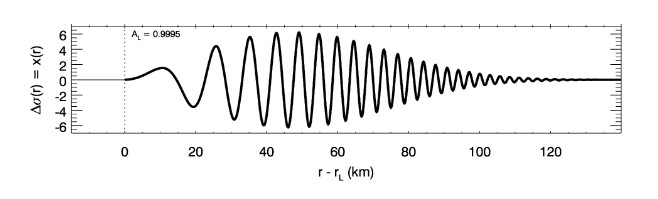
\includegraphics[width=1.0\textwidth]{Linear_Density_WM.jpg}
\caption{Synthetic density-wave radial profile generated by Equation (1) for a case of $m>0$ (prograde) \cite{Tiscareno_2007}.} \label{fig:my_label}
\end{figure}


%.................................................................




%       LAPLKACE COEFFICIENT WORK

\begin{align*}
\int_0^{2 \pi} \frac{\cos mx}{\sqrt{1 - 2 \alpha \cos x + \alpha^2}} dx &= \int_0^{2 \pi} \frac{\cos mx}{\alpha \sqrt{1 - k^2 \sin^2 x}} dx \\
&= \frac{1}{\alpha} \int_0^{2 \pi} \frac{\cos mx}{\sqrt{1 - k^2 \sin^2 x}} dx \\
&= \frac{1}{\alpha} F(2 \pi, k)
\end{align*}

$F(x, k) = \int_0^x \frac{1}{\sqrt{1 - k^2 \sin^2 u}} du$





%.................................................................................






%................................................................................


\bibliographystyle{plain}\bibliography{reference}

\end{document}








